	\documentclass[../pfc.tex]{subfiles}

	
	\begin{document}
	
La fase de análisis y el proceso de Ingeniería de Requisitos, parten básicamente de dos contextos bien diferenciados:\\
-Por una parte de las reuniones mantenidas con el cliente, en este caso la AECC.

-Por otra parte del libro que utiliza la AECC llamado \textbf{MIS CUIDADOS, DIARIO DE SALUD DE UN SUPERVIVIENTE DE CANCER} y que se utiliza de manera general sobre enfermos de cáncer que han superado esta enfermedad y sobre otros que todavía la siguen padeciendo.\\\\
	
	\section{¿El porqué?}
	
	Desde el punto de vista de la definición clásica:
	
	La ingeniería del software es el proceso formal de desarrollo de software en el que las necesidades del usuario se traducen en requisitos, estos se transforman en diseño que se implementa en código que se prueba, documenta y se certifica para su uso operativo. Según la definición del IEEE la ingeniería del software se define como “(1) la aplicación de un método sistemático, disciplinado y cuantificable al desarrollo, operación y mantenimiento de software, esto es, la aplicación de la ingeniería al software” y “(2) el estudio de los métodos de (1)”\\
	
	El proceso requiere una metodología con 5 etapas:
	
	Análisis de requisitos: Se extraen los requisitos del producto de software. En esta etapa la habilidad y experiencia en la ingeniería del software es crítica para reconocer requisitos incompletos, ambiguos o contradictorios.\\
	Usualmente el cliente/usuario tiene una visión incompleta/inexacta de lo que necesita y es necesario ayudarle para obtener la visión completa de los requerimientos.  El contenido de comunicación en esta etapa es muy intenso ya que el objetivo es eliminar la ambigüedad en la medida de lo posible.\\
	Partiendo de un exhaustivo estudio de las funcionalidades que podrian resultar útiles para los pacientes de Cancer, y de acuerdo con las especificaciones de la AECC hemos decidido incluir en la misma las siguientes:\\

	\section{Explicación detallada de las funcionalidades de la aplicación}


	\textbf{AVATAR}
	
	Editar el perfil, Foto, nombre, apellidos, edad, cumpleaños... (1 pantalla), ¿Grupo sanguineo y alergenos tampoco estaría mal pero es informacion de otro nivel LOPD?
	
	PROYECTO AMPLIACION (asignar un agente personalizado para poder atender de manera personalizada al paciente Superviviente)\\
	

	\textbf{PRINCIPAL}
	
	Vista de Rutina proxima, citas, Se debería ver lo que realmente interesa ¿Noticias AECC tipo RSS, Twitter, Facebook? (1 pantalla)\\
	

	\textbf{HORARIO}
	
	Vista dia, mes, con las actividades, citas, ¿Cumpleaños, aniverssario de enfermedad...?  
	al pinchar en una hora, dia, se podrá añadir rutina o cita, iria a la correspondiente lista de creacion de una nueva (1 pantalla)
	
	Deberian aparecer las citas y rutinas ocupando el espacio destinado a la duracion de las mismas.
	
	Revisar esta página
	https://code.google.com/p/yadview/\\
	

	\textbf{RUTINA}
	Lista de rutinas, desde la propia vista se podrán añadir rutinas, al pulsar sobre la opción correspondiente nos llevará al listado de estás opciones añadiendose así.
	
	Se podra ordenar por fecha, asc y desc, duracion de la actividad asc y desc pero sobre todo se podrá ordenar por satisfaccion de la misma.
	
	Añadir rutina, , en esta pantalla se permite ver al pinchar sobre el propio item de la lista ,editar, o pulsando el botón añadir del final de la lista crear una nueva,
	Valorar si deberiamos gestionar la repeticion de los elementos					
	dentro de la rutina (añadir) se podrán añadir personajes y asignar una alarma personalizable (avisar) con antelacion, se puede ver sin editar(2 pantallas)
	con una hora de aviso, hora de empiece de la actividad. Duración de las misma en horas, satisfaccion de 0 a 10
	
	Dentro se va a valorar tambien la satisfacción personal que se produce al hacer esto, podrá ser de 0 a 10
	
	AMPLIACION DE PROYECTO: Poder variar los avisos para que se hagan de manera repetitiva, por ejemplo repetir de manera semanal los jueves al estilo TICK TICK, llamarlo actividades en vez de Rutina\\ 
	

	\textbf{CITAS}
	
	Lista de citas Nombre de la cita, fecha y hora.
	Desde el propio item de la lista se podran añadir medicamentos, personas, sintomas y/o pruebas, al pulsar sobre la opción correspondiente nos llevará al listado de estás opciones añadiendose así.
	
	Añadir cita, en esta pantalla se permite ver al pinchar sobre el propio item de la lista ,editar, o pulsando el botón añadir del final de la lista crear una nueva, 
	dentro de la cita (añadir) se podrán añadir ubicación, personajes, medicamentos, pruebas y sintomas y asignar una alarma personalizable con fecha y hora (avisar) con antelacion.
	se puede ver sin editar
	
	Deberíamos añadir duración?
	
	Valorar si deberiamos gestionar la repeticion de los eventos
	
	¿En la ubicación se podria comunicar con google maps?
	
	¿Deberiamos mostrar en el item de la cita si ya poseee personas, pruebas, sintomas o medicacion?
	
	PROYECTO AMPLIACION Poder exportar e importar a google maps, conectar la ubicacion con google maps para poder ir\\
	
	
	\textbf{MEDICACION}
	Lista de medicamentos, lista de los medicamentos que tengamos con el boton de añadir al final y en la barra la posibilidad de ordenar en principio por orden ascendente o descendente,
	al pinchar sobre el elemento se visualiza, en las opciones de cada elemento se puede añadir a la cita, editar y borrar (confirmacion para borrar)
	
	Añadir medicamento, , en esta pantalla se permite ver al pinchar sobre el propio item de la lista ,editar, o pulsando el botón añadir del final de la lista crear una nueva, 
	dentro del medicamento (añadir) se podrá asignar una foto personalizable, o bien hacerla o añadirla de la galeria, viene una por defecto
	nombre, descripcion, 
	una alarma personalizable que avisar con antelacion, fecha inicio, hora inicio, fecha fin, hora fin, repetir cada tantas horas, dias, semanas, (esto se valorará)

	REVISAR LA FUNCION DE ALARMA EN ANDROID http://developer.android.com/reference/android/app/AlarmManager.html
	boton guardar 
	se puede ver sin editar, 
	dentro de la edición y visionado se podra añadir a una cita
	Se puede añadir el numero de medicamentos al drawer (se estudiará)
	
	PROYECTO AMPLIACION Llevar el stock de lo que lleva consumido el paciente y generar alertas para cuando se le acabe, duplicar tratamiento, para ahorrar trabajo, opciones de dosis.\\
	
	
	\textbf{PERSONAJES}
	
	Lista de personajes que tengamos con el boton de añadir al final y en la barra la posibilidad de ordenar en principio por orden ascendente o descendente,
	al pinchar sobre el elemento se visualiza, 
	en las opciones de cada elemento se puede añadir a la cita, a la rutina, editar y borrar confirmacion para borrar
	
	Añadir persona, , en esta pantalla se permite ver al pinchar sobre el propio item de la lista ,editar, o pulsando el botón añadir del final de la lista crear una nueva, 
	dentro de la persona(añadir) se podrá asignar una foto personalizable, o bien hacerla o añadirla de la galeria, viene una por defecto
	nombre apellidos, puesto / tipo (doctor, oncologo, cirujano, farmaceutico, enfermero, medico cabecera, familiar, amigo,AECC, otro), telefono (posibilidad de llamar desde la visualizacion)
	se puede ver sin editar, dentro de la edición y visionado se podra añadir a una cita, o a una rutina ejemplo (paseo por la playa) o a cita con el oncólogo
	Se puede añadir el numero al drawer
	
	PROYECTO AMPLIACION llevarnos ese contacto a la agenda o traernosle de ella\\
	
	
	\textbf{PRUEBAS}
	
	Lista de personajes que tengamos con el boton de añadir al final y en la barra la posibilidad de ordenar en principio por orden de fecha ascendente o descendente,
	al pinchar sobre el elemento se visualiza, 
	en las opciones de cada elemento se puede añadir a la cita, editar y borrar confirmacion para borrar
	
	Añadir prueba, , en esta pantalla se permite ver al pinchar sobre el propio item de la lista ,editar, o pulsando el botón añadir del final de la lista crear una nueva, 
	dentro de la prueba (añadir) se podrá asignar una foto personalizable, o bien hacerla o añadirla de la galeria, viene una por defecto
	nombre, descripcion,
	fecha y hora de la misma
	se puede ver sin editar, dentro de la edición y visionado se podra añadir a una cita por ejemplo visita al oncólogo
	Se puede añadir el numero al drawer
	
	PROYECTO AMPLIACION poder subir documentos tipo pdf para no depender de la fotografia solo, llevar estadísticas\\
	
	
	\textbf{SINTOMAS}
	
	Lista de síntomas que tengamos con el boton de añadir al final y en la barra la posibilidad de ordenar en principio por orden de fecha ascendente o descendente,
	al pinchar sobre el elemento se visualiza, 
	en las opciones de cada elemento se puede añadir a la cita, editar y borrar confirmacion para borrar
	
	Añadir sintoma, , en esta pantalla se permite ver al pinchar sobre el propio item de la lista ,editar, o pulsando el botón añadir del final de la lista crear una nueva, 
	dentro de la prueba (añadir) se podrá asignar una foto personalizable, o bien hacerla o añadirla de la galeria, viene una por defecto
	nombre, descripcion de los sintomas,
	fecha y hora de la misma
	se puede ver sin editar, dentro de la edición y visionado se podra añadir a una cita por ejemplo visita al oncólogo
	Se puede añadir el numero al drawer
	
	PROYECTO AMPLIACION poder subir documentos tipo pdf para no depender de la fotografia solo, llevar estadísticas, poder conectar con los centros de salud, hospitales, \\
	
	
	\textbf{RECURSOS}
	Dentro de los resursos aparece meditacion con musica relajante e instrucciones para ello
	consejos generales, de alimentacion, de vida, de salud...
	telefonos de interés generales (DEBEMOS DECIDIR SI SE PUEDEN PERSONALIZAR)
	Noticias (podemos añadir el blog de la AECC o la cuenta de twitter que no esta nada mal)
	
	
	\textbf{AJUSTES}
	Editar el perfil, 
	tamaño de letra, 	
	tono para alertas de citas y rutinas, 
	color del led de notificación, 
	posibilidad de feedback,
	quienes somos o motivaciones (¿? pantallas)\\\\

	
	\section{Documento de Análisis}
	
	Aunque utilizamos una metología ágil, hay puntos en los que no nos podemos separar de la metodología tradicional.
			
	Es difícil capturar todos los requisitos a partir de unas cuantas reuniones, para nuestro caso, pudimos contar con la ayuda del libro "Mis Cuidados, diario de salud para supervivientes de cáncer"
			
	Una de las ventajas de utilizar este primer tipo de metodología, es el de poder adaptar de una manera mucho más eficiente los recursos a las fechas y a los requisitos, y poder modificar estos requisitos de manera "ágil" debido al panorama cambiante que podemos tener de cara al cliente.
			
	\begin{figure}
		\centering
		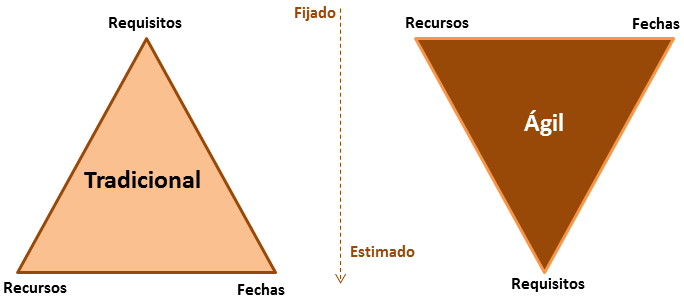
\includegraphics[width=0.5\linewidth]{../images/paradigmaRequisitos}
		\caption{Paradigma captura de requisitos método tradicional vs. ágil}
		\label{fig:paradigmaRequisitos}
	\end{figure}
			
			
	\subsection{Descripción de objetivos de manera detallada}
	
	
	\textbf{OBJ-001}	La aplicacion debera poder administrar un perfil de usuario\\*
	
		\begin{table}[!hbt]
			\centering
			\begin{tabular}[t]{|l|l|}
				\hline \textbf{OBJ-001} & \textbf{PERFIL DE USUARIO} \\*
				\hline\hline \textbf{Versión} & 1.0 \\ *
				\hline\textbf{Autores} 	& Fernando Santa Olaya Rodríguez \\*
				& Rubén Toquero González\\*
				\hline \textbf{Descripción} & La aplicacion debera poder administrar un perfil de usuario\\* 
				\hline \textbf{Subobjetivos} & El usuario padrá introducir una foto, nombre, fecha de nacimiento \\* 
				\hline \textbf{Importacia} & Importante \\* 			
				\hline \textbf{Urgencia} & Inmediatamente \\* 
				\hline \textbf{Estado} & En construcción \\* 
				\hline \textbf{Estabilidad} & Estable \\* 
				\hline \textbf{Comentarios} & En la cabecera del drawer aparecerá el nombre y la foto \\* 
				\hline 
			\end{tabular}
			\caption{Menú drawer.}
			\label{tabla:req001}
		\end{table}
	
	\textbf{OBJ-002}	La aplicacion será facil de navegar para usuarios no avanzados\\*
	
	\textbf{OBJ-003}	La aplicacion facilitará la gestion de las actividades diarias de un usuario (medicas/rutinarias)\\*
	
	\textbf{OBJ-004}	La aplicacion permitirá gestionar de manera organizada las citas médicas de un usuario\\*
	
	\textbf{OBJ-005}	La aplicacion permitirá gestionar de manera organizada las rutinas diarias de un usuario\\*
	
	\textbf{OBJ-006}	La aplicacion permitirá gestionar de manera organizada los medicamentos asignados a un usuario\\*
	
	\textbf{OBJ-007}	La aplicacion permitirá gestionar de manera organizada los personajes que interactuan en las
	 actividades de un usuario\\*
	
	\textbf{OBJ-008}La aplicacion permitirá gestionar de manera organizada los síntomas que acontecen a un usuario\\*
	
	\textbf{OBJ-009}	La aplicacion permitirá gestionar de manera organizada las pruebas médicas a las que se somete un
	 usuario\\*
	
	\textbf{OBJ-010}	La aplicacion proporcionará recursos de ayuda para el bienestar del usuario\\*
	
	\textbf{OBJ-011}	La aplicación permitirá ajustes que mejoren la experiencia del usuario\\*
	
	\textbf{OBJ-012}	La aplicación deberá tener una base de datos para almacenar toda la informacion del usuario\\*
	
	\textbf{OBJ-013}	La aplicación deberá contar con un manual de usuario para facilitar su comprension y uso\\*
	
	\textbf{OBJ-014}	La aplicación soportará el mayor número de dispositivos android posibles\\*
	
	\textbf{OBJ-015}	La aplicación será de verdadera ayuda para usuarios incluidos dentro de la iniciativa de la AECC\\*
	
	\textbf{OBJ-016}	La aplicación se integrará perfectamente dentro de la iniciativa de la AECC\\*
	
	

	
	
	\subsection{Captura de Requisitos}
	
	Como consecuencia de las diferentes reuniones realizadas con el cliente se elabora un
	documento de especificación de requisitos con el propósito de describir las funcionalidades
	necesarias para poder validar el producto final.\\*
	
	\subsubsection{Requisitos de información}
			
	
	\subsubsection{Requisitos Funcionales}
	
	A continuación se describirán los requisitos para este proyecto. Se tendrán dos tipos de
	requisitos: requisitos funcionales, que serán aquellos obtenidos a partir de los objetivos principales
	y secundarios del apartado anterior; y requisitos no funcionales, obtenidos de las especificaciones
	citadas a lo largo de la memoria y que precisen ser descritas como requisitos.\\*
	
	Este tipo de requisitos declaran los servicios que debe proporcionar el sistema, como debe
	reaccionar a una entrada particular y cómo se debe de comportar ante situaciones particulares.
	Describen el funcionamiento del sistema.\\*
	
	Los requisitos de información llevarán un nombre descriptivo y un número para identificarlos.
	Este número tendrá el formato IRQ - <id> donde id será el número del requisito de información.
	Además se indicarán los requisitos asociados, una descripción y cualquier información que sea
	relevante para una mayor claridad.\\*
	
	Los requisitos funcionales que debe cumplir el sistema son los siguientes\\*
	
	
	\textbf{FRQ-001}	El usuario podra acceder a un menú de navegación	\textbf{OBJ-002}\\*

	\begin{table}[!hbt]
		\centering
		\begin{tabular}[t]{|l|l|}
			\hline \textbf{FRQ-001} & \textbf{DRAWER MENÚ} \\*
			\hline\hline \textbf{Versión} & 1.0 \\ *
			\hline\textbf{Autores} 	& Fernando Santa Olaya Rodríguez\\*
			& Rubén Toquero González\\*
			\hline \textbf{Dependencias} & OBJ-002\\* 			
			\hline \textbf{Descripción} & El usuario podrá acceder a un menú de navegación \\* 
			\hline \textbf{Importancia} & Vital \\* 
			\hline \textbf{Urgencia} & Inmediatamente \\* 
			\hline \textbf{Estado} & En construcción \\* 
			\hline \textbf{Estabilidad} & Estable \\* 
			\hline \textbf{Comentarios} & El menú será visible al desplazar el dedo de izquierda a derecha de la pantalla \\* 
			\hline 
		\end{tabular}
		\caption{Menú drawer.}
		\label{tabla:req001}
	\end{table}
	
	
	\textbf{FRQ-002}	El usuario podrá introducir sus datos personales en la aplicación 	\textbf{OBJ-001}
	
	\textbf{FRQ-003}	El usuario podra visualizar sus datos personales	\textbf{OBJ-001}
	
	\textbf{FRQ-004}	Es usuario podrá ver/editar sus datos personales	\textbf{OBJ-001}\\*
	
	
	
	\textbf{FRQ-005}	El usuario al acceder a la aplicación podra visualizar de un vistazo su actividad para hoy 		\textbf{OBJ-003}
	
	\textbf{FRQ-006}	El usuario podrá acceder desde la pantalla principal a sus citas medicas	\textbf{OBJ-003 OBJ-004}
	
	\textbf{FRQ-007}	El usuario podrá acceder desde la pantalla principal a sus rutinas diarias	\textbf{OBJ-003}  \textbf{OBJ-005}\\*					
	
	
	AFECTADAS POR EL OBJETIVO \textbf{OBJ-004}\\*
	\textbf{FRQ-008}	La aplicación mostrará una vista del dia actual con actividades del usuario de ese dia (citas y rutinas)
	
	\textbf{FRQ-009}	La aplicación mostrará una vista del mes actual para las actividades del usuario de ese mes (citas y rutinas)	\textbf{OBJ-003}
	
	\textbf{FRQ-010}	El usuario podrá añadir una cita desde cualquiera de las vistas mensual/diaria
	
	\textbf{FRQ-011}	El usuario podrá añadir una rutina para ese dia desde cualquiera de las vistas mensual/diaria
	
	\textbf{FRQ-012}	El usuario podrá visualizar/editar la cita desde cualquiera de esas vistas
	
	\textbf{FRQ-013}	El usuario podrá visualizar/editar la rutina desde cualquiera de esas vistas\\*
	
	
	AFECTADOS POR EL OBJETIVO 	\textbf{OBJ-004}\\*
	
	\textbf{FRQ-014}	El usuario podrá acceder a la lista de citas medicas
	
	\textbf{FRQ-015}	El usuario podrá añadir desde la lista una nueva cita medica
	
	\textbf{FRQ-016}	El usuario podrá añadir alertas y notificaciones a una cita médica
	
	\textbf{FRQ-017}	El usuario podrá añadir personajes a una cita medica
	
	\textbf{FRQ-018}	El usuario podrá añadir pruebas a una cita medica
	
	\textbf{FRQ-019}	El usuario podrá añadir medicamentos a una cita medica
	
	\textbf{FRQ-020}	El usuario podrá añadir duración a una cita médica
	
	\textbf{FRQ-021}	El usuario podrá añadir síntomas a una cita medica
	
	\textbf{FRQ-022}	El usuario podrá visualizar/editar la cita medica\\*
	
	
	
	AFECTADOS POR EL OBJETIVO 	\textbf{OBJ-005}\\*
	\textbf{FRQ-023}	El usuario podrá acceder a la lista de rutinas
	
	\textbf{FRQ-024}	El usuario podrá añadir desde la lista una nueva rutina
	
	\textbf{FRQ-025}	El usuario podrá añadir alertas y notificaciones a una rutina
	
	\textbf{FRQ-026}	El usuario podrá añadir duración a una rutina
	
	\textbf{FRQ-027}	El usuario podrá añadir personajes a una rutina
	
	\textbf{FRQ-028}	El usuario podrá visualizar/editar la rutina\\*
	
	
	
	
	AFECTADOS POR EL OBJETIVO 	\textbf{OBJ-006}\\*
	\textbf{FRQ-029}	El usuario podrá acceder a la lista de medicamentos
	
	\textbf{FRQ-030}	El usuario podrá añadir desde la lista un nuevo medicamento
	
	\textbf{FRQ-031}	El usuario podra añadir información importante respecto a ese medicamento
	
	\textbf{FRQ-032}	El usuario podrá añadir alertas y notificaciones a medicamento
	
	\textbf{FRQ-033}	El usuario podrá visualizar/editar el medicamento\\*
	
	
	AFECTADOS POR EL OBJETIVO 	\textbf{OBJ-007}
	
	\textbf{FRQ-034 A FRQ-049}	Lo mismo con personajes, sintomas, pruebas\\*
	
	
	
	AFECTADOS POR EL OBJETIVO 	\textbf{OBJ-010}\\*
	\textbf{FRQ-050}	El usuario podrá acceder a recursos relaccionados con el autocontrol y la meditacion
	
	\textbf{FRQ-051}	El usuario tendrá acceso a telefonos de interés
	
	\textbf{FRQ-052}	El usuario tendrá acceso a consejos que le proporcionen bienestar
	
	\textbf{FRQ-053}	El usuario tendrá acceso a noticias relativas a la AECC\\*
	
	
	
	\textbf{FRQ-054}	La aplicación notificará al paciente a peticion citas y rutinas\\*
	
	\textbf{FRQ-055}	Las listas seran ordenable segun diferentes criterios\\*
	
	
	AFECTADOS POR EL OBJETIVO 	\textbf{OBJ-011}\\*
	\textbf{FRQ-056}	La aplicacion contendrá ajustes que faciliten su manejo al usuario\\*
	
	
	
	

	
	
		
	
		 
		
	


	\subsubsection{Requisitos No Funcionales}
	
	Este tipo de requisitos define las propiedades emergentes del sistema, tales como el tiempo de
	respuesta, las necesidades de almacenamiento, la fiabilidad.\\*
	
	Pueden especificar también la utilización de una herramienta CASE en particular, un lenguaje
	de programación o un método del desarrollo.\\*
	
	En este apartado se detalla el catálogo de requisitos no funcionales. Estos requisitos pueden
	ser más críticos que los requisitos funcionales, ya que son a los que normalmente debe apuntar la
	arquitectura y si estos no son cumplidos, el software puede no funcionar o el cliente simplemente
	no acepta el producto.\\*
	
	Estos requisitos se puede decir que no están relacionados directamente con la funcionalidad
	del sistema. Con esto no se pretende decir que no sean necesarios para la funcionalidad del sistema,
	pero sí que no pueden asociarse a ningún caso de uso en particular. Hay distintas categorías y tipos
	de requisitos no funcionales: hardware, plataforma software, comunicaciones, de interfaz, de
	seguridad, de control de concurrencia, de persistencia…etc.\\*
	
	Los requisitos no funcionales llevarán un nombre descriptivo y un número para identificarlos.
	Este número tendrá el formato NFRQ - <id> donde id será el número del requisito de información.
	Además se indicará una descripción y cualquier información que sea relevante para una mayor
	claridad.\\*
	
	Algunos requisitos no funcionales identificados para el desarrollo del presente proyecto son
	los siguientes:\\*

	AFECTADOS POR EL OBJETIVO 	\textbf{OBJ-015}\\*
		
	\textbf{NFRQ-001}		La aplicacion será un apoyo y una ayuda para el paciente\\*
	
	
	AFECTADOS POR EL OBJETIVO 	\textbf{OBJ-016}\\*
		
	\textbf{NFRQ-002}		La aplicación debe ser coherente con el programa de Diario de Salud de la AECC.
	
	
	AFECTADOS POR EL OBJETIVO 	\textbf{OBJ-013 OBJ-015}\\*		
	\textbf{NFRQ-003}		La aplicacion sera amigable para usuarios no avanzados
	
	
	AFECTADOS POR EL OBJETIVO 	\textbf{OBJ-016}\\*	
	\textbf{NFRQ-004}		La aplicacion cumplira las guias de estilo fijadas por la AECC
	
	
	AFECTADOS POR EL OBJETIVO 	\textbf{OBJ-015}\\*		
	\textbf{NFRQ-005}		La aplicación proporcionará recursos de valor para los enfermos de cancer.
	
	
		
	\textbf{NFRQ-006}		La aplicación será mantenible y escalable a petición del cliente.


	AFECTADOS POR EL OBJETIVO 	\textbf{OBJ-004}\\*	
	\textbf{NFRQ-007}		La aplicación facilitara las visitas médicas


	AFECTADOS POR EL OBJETIVO 	\textbf{OBJ-005}\\*			
	\textbf{NFRQ-008}		La aplicacion incentivará la realizacion de actividades placenteras para el paciente


	AFECTADOS POR EL OBJETIVO 	\textbf{OBJ-003}\\*		
	\textbf{NFRQ-009}		La aplicacion facilitara la organizacion de los compromisos del usuario


		
	\textbf{NFRQ-010}		La aplicación será segura y confiable
	
	
	\textbf{NFRQ-011}		La aplicación estará finalizada antes del dia 9 de septiembre


		
	

	\subsection{Identificación de actores}
		
	\subsection{Diagrama de casos de uso }
		



	\subsection{Descripción de Casos de Uso}
	
	CASOS DE USO\\*
	
	\textbf{CU-001} PERFIL DE USUARIO - Inserción de perfil\\*
	
	\begin{table}[!hbt]
		\centering
		\begin{tabular}[t]{|p{3cm}|p{9.5cm}|}
				\hline \textbf{CU-001} & \textbf{PERFIL DE USUARIO- INSERCIÓN} \\*
				\hline\hline \textbf{Versión} & 1.0 \\ *
				\hline\hline \textbf{Fecha} & 23/07/2015 \\ *
				\hline\textbf{Actores} 	& Usuario\\*
				\hline \textbf{Objetivo} & Incluir en el sistema los datos personales del usuario\\* 			
				\hline \textbf{Precondición} & Los datos del usuario están sin completar \\* 
				\hline \textbf{Flujo normal} & 1.- Desplegamos el menú drawer \\* 
											 & 2.- Pulsamos el circulo que está al principio del menú \\*	
											 & 3.- Rellenamos los datos personales del usuario\\*	
				\hline \textbf{Flujo alternativo} & 1.- Desplegamos el menú drawer \\* 
 												  & 2.- Pulsamos la opcion ajustes \\*	
												  & 3.- Pulsamos la opción en pantalla "Perfil" \\*	
												  & 3.- Rellenamos los datos personales del usuario \\*	
				\hline \textbf{Postcondición} & El usuario posee sus datos personales en la aplicación \\* 
				\hline \textbf{Comentarios}   & A la hora de introducir la fotografía dentro de los datos personales, podrá elegir entre las que tenga en la galeria del propio terminal o acceder a la aplicación de cámara para hacer una nueva fotografía\\*
				\hline
			\end{tabular}
			\caption{Prefil de usuario - Inserción}
			\label{tabla:caso001}
	\end{table}
	
	
	
	\textbf{CU-002}PERFIL DE USUARIO - edicion de perfil\\*
	
	\begin{table}[!hbt]
		\centering
		\begin{tabular}[t]{|p{3cm}|p{9.5cm}|}
			\hline \textbf{CU-002} & \textbf{PERFIL DE USUARIO - EDICIÓN} \\*
			\hline\hline \textbf{Versión} & 1.0 \\ *
			\hline\hline \textbf{Fecha} & 24/07/2015 \\ *
			\hline\textbf{Actores} 	& Usuario\\*
			\hline \textbf{Objetivo} & Modificar en el sistema los datos personales del usuario\\* 			
			\hline \textbf{Precondición} & Los datos del usuario existen en la aplicación \\* 
			\hline \textbf{Flujo normal} & 1.- Desplegamos el menú drawer \\* 
			& 2.- Pulsamos el circulo que está al principio del menú \\*	
			& 3.- Rellenamos los datos personales del usuario\\*	
			\hline \textbf{Flujo alternativo} & 1.- Desplegamos el menú drawer \\* 
			& 2.- Pulsamos la opción ajustes \\*	
			& 3.- Pulsamos la opción en pantalla "Perfil" \\*	
			& 3.- Rellenamos los datos personales del usuario \\*	
			\hline \textbf{Postcondición} & El usuario posee sus datos personales modificados\\* 
			\hline \textbf{Comentarios}   & El usuario puede a su elección dejar los datos tal y como estuviesen en un principio\\*
			\hline
		\end{tabular}
		\caption{Perfil de usuario - Edición}
		\label{tabla:caso002}
	\end{table}
	

	
	\textbf{CU-002A}	PERFIL DE USUARIO - visualizacion de perfil\\*

	La visualización del perfil pude ser un caso de uso que converge con el anterior, comparten pre y post condición, y el flujo de acceso es prácticamente el mismo (Se estudiará)

	
	
		
	\textbf{CU-003}	PERFIL DE USUARIO - Borrado de perfil\\*

	\begin{table}[!hbt]
		\centering
		\begin{tabular}[t]{|p{3cm}|p{9.5cm}|}
			\hline \textbf{CU-003} & \textbf{PERFIL DE USUARIO - BORRADO} \\*
			\hline\hline \textbf{Versión} & 1.0 \\ *
			\hline\hline \textbf{Fecha} & 24/07/2015 \\ *
			\hline\textbf{Actores} 	& Usuario\\*
			\hline \textbf{Objetivo} & Borrar del sistema los datos personales del usuario\\* 			
			\hline \textbf{Precondición} & Los datos del usuario existen en la aplicación \\* 
			\hline \textbf{Flujo normal} & 1.- Desplegamos el menú drawer \\* 
			& 2.- Pulsamos el circulo que está al principio del menú \\*	
			& 3.- Rellenamos los datos personales del usuario\\*	
			\hline \textbf{Flujo alternativo} & 1.- Desplegamos el menú drawer \\* 
			& 2.- Pulsamos la opcion ajustes \\*	
			& 3.- Pulsamos la opción en pantalla "Perfil" \\*	
			& 3.- Rellenamos los datos personales del usuario \\*	
			\hline \textbf{Postcondición} & El usuario ya NO posee sus datos personales en la aplicación \\* 
			\hline \textbf{Comentarios}   &  \\*
			\hline
		\end{tabular}
		\caption{Perfil de usuario - Borrado}
		\label{tabla:caso003}
	\end{table}
	
	
	

	\textbf{CU-004}	CITA MEDICA - Inserción de cita médica\\*
	
	\begin{table}[!hbt]
		\centering
		\begin{tabular}[t]{|p{3cm}|p{9.5cm}|}
			\hline \textbf{CU-004} & \textbf{CITA MÉDICA - INSERCIÓN} \\*
			\hline\hline \textbf{Versión} & 1.0 \\ *
			\hline\hline \textbf{Fecha} & 27/07/2015 \\ *
			\hline\textbf{Actores} 	& Usuario\\*
			\hline \textbf{Objetivo} & Insertar en la aplicación una cita médica que tiene el usuario\\* 			
			\hline \textbf{Precondición} & La cita médica no existe en la aplicación\\* 
			\hline \textbf{Flujo normal} & 1.- Desplegamos el menú drawer \\* 
			& 2.- Pulsamos la opción CITA MEDICA\\*	
			& 3.- Pulsamos el icono +\\*	
			& 4.- Rellenamos los datos pertinentes de la cita médica\\*	
			\hline \textbf{Flujo alternativo} & 1a.- Desplegamos el menú drawer \\* 
			& 2a.- Pulsamos la opción Principal \\*	
			& 3a.- Elegimos la opción "añadir cita" al pulsar el icono +\\*	
			& 4a.- Completamos los datos de la cita\\*	
			& 1b.- Desplegamos el menú drawer \\* 
			& 2b.- Pulsamos la opción Horario \\*	
			& 3b.- Elegimos la opción "añadir cita" al pulsar el icono +\\*	
			& 4b.- Completamos los datos de la cita\\*	
			& 5b.- Sobre la vista mensual se puede añadir una cita al pulsar sobre el dia del mes y continuando con el flujo anteriormente indicado\\*	
			\hline \textbf{Postcondición} & El usuario ya posee los datos de la cita en la aplicación \\* 
			\hline \textbf{Comentarios}   & Los valores de la fecha de la cita y el nombre de la misma son obligatorios, en caso de no ser rellenados, el sistema avisará con un mensaje de error y no se podrá guardar la misma.\\*
			\hline
		\end{tabular}
		\caption{Cita médica - Inserción}
		\label{tabla:caso004}
	\end{table}




	\textbf{CU-005}	CITA MEDICA - edicion de cita médica\\*
	
		\begin{table}[!hbt]
			\centering
			\begin{tabular}[t]{|p{3cm}|p{9.5cm}|}
				\hline \textbf{CU-005} & \textbf{CITA MÉDICA - Edición} \\*
				\hline\hline \textbf{Versión} & 1.0 \\ *
				\hline\hline \textbf{Fecha} & 27/07/2015 \\ *
				\hline\textbf{Actores} 	& Usuario\\*
				\hline \textbf{Objetivo} & Editar una cita médica que ya posee el usuario\\* 			
				\hline \textbf{Precondición} & La cita médica existe en la aplicación\\* 
				\hline \textbf{Flujo normal} & 1.- Desplegamos el menú drawer \\* 
				& 2.- Pulsamos la opción CITA MEDICA\\*	
				& 3.- Pulsamos sobre los tres puntos a la derecha de la cita médica que queremos editar\\*	
				& 4.- Seleccionamos la opción editar\\*	
				& 5.- Modificamos los datos pertinentes de la cita médica que queramos cambiar\\*	
				\hline \textbf{Flujo alternativo} & 1.- Desplegamos el menú drawer \\* 
				& 2.- Pulsamos la opcion Horario \\*	
				& 3.- Pulsamos sobre el icono de los tres puntos de cita que queramos modificar \\*	
				& 4.- Elegimos la opcion "editar"\\*	
				& 5.- Modificamos los datos de la cita\\*	
				\hline \textbf{Postcondición} & El usuario ya posee los nuevos datos modificados de la cita en la aplicación \\* 
				\hline \textbf{Comentarios}   & Los valores de la fecha de la cita y el nombre de la misma son obligatorios, en caso de no ser completados, el sistema avisará con un mensaje de error y no se podrá guardar la misma.\\*
				\hline
			\end{tabular}
			\caption{Cita médica - Edición}
			\label{tabla:caso005}
		\end{table}
		
	
	\textbf{CU-006}	CITA MEDICA - visualizacion de cita médica\\*
	
	
	
	\textbf{CU-007}	CITA MEDICA - borrado de cita médica\\*
	
		\begin{table}[!hbt]
			\centering
			\begin{tabular}[t]{|p{3cm}|p{9.5cm}|}
				\hline \textbf{CU-005} & \textbf{CITA MÉDICA - Borrado} \\*
				\hline\hline \textbf{Versión} & 1.0 \\ *
				\hline\hline \textbf{Fecha} & 27/07/2015 \\ *
				\hline\textbf{Actores} 	& Usuario\\*
				\hline \textbf{Objetivo} & Borrar una cita médica que ya posee el usuario\\* 			
				\hline \textbf{Precondición} & La cita médica existe en la aplicación\\* 
				\hline \textbf{Flujo normal} & 1.- Desplegamos el menú drawer \\* 
				& 2.- Pulsamos la opción CITA MEDICA\\*	
				& 3.- Pulsamos sobre los tres puntos a la derecha de la cita médica que queremos eliminar dentro del listado\\*	
				& 4.- Seleccionamos la opción eliminar\\*	
				\hline \textbf{Flujo alternativo} & 1.- Desplegamos el menú drawer \\* 
				& 2.- Pulsamos la opción Horario \\*	
				& 3.- Pulsamos sobre el icono de los tres puntos de cita que queramos eliminar \\*	
				& 4.- Elegimos la opción "Eliminar"\\*	
				& 5.- Modificamos los datos de la cita\\*	
				\hline \textbf{Postcondición} & El usuario ya posee los nuevos datos modificados de la cita en la aplicación \\* 
				\hline \textbf{Comentarios}   & Los valores de la fecha de la cita y el nombre de la misma son obligatorios, en caso de no ser completados, el sistema avisará con un mensaje de error y no se podrá guardar la misma.\\*
				\hline
			\end{tabular}
			\caption{Cita médica - Edición}
			\label{tabla:caso007}
		\end{table}
		
		
	
	\textbf{CU-008}	RUTINA - insercion de rutina\\*
	
	\textbf{CU-009}	RUTINA - edicion de rutina\\*
	
	\textbf{CU-010}	RUTINA - visualizacion de rutina\\*
	
	\textbf{CU-011}	RUTINA - borrado de rutina\\*
	
	
	
	\textbf{CU-012}	MEDICAMENTO - insercion de medicamento\\*
	
	\textbf{CU-013}	 MEDICAMENTO - edicion de medicamento\\*
	
	\textbf{CU-014}	 MEDICAMENTO - visualizacion de medicamento\\*
	
	\textbf{CU-015}	 MEDICAMENTO - borrado de medicamento\\*
	
	
	
	\textbf{CU-016}	 PERSONAJE - insercion de personajes\\*
	
	\textbf{CU-017}	 PERSONAJE - edicion de personajes\\*
	
	\textbf{CU-018}	 PERSONAJE - visualizacion de personajes\\*
	
	\textbf{CU-019}	 PERSONAJE - borrado de personajes\\*
	
	
	
	\textbf{CU-020}	 SINTOMA - insercion de síntoma\\*
	
	\textbf{CU-021}	 SINTOMA - edicion de síntoma\\*
	
	\textbf{CU-022}	 SINTOMA - visualizacion de síntoma\\*
	
	\textbf{CU-023}	 SINTOMA - borrado de síntoma\\*
	
	
	
	\textbf{CU-024}	 PRUEBA -insercion de pruebas\\*
	
	\textbf{CU-025}	 PRUEBA -edicion de pruebas\\*
	
	\textbf{CU-026}	 PRUEBA -visualizacion de pruebas\\*
	
	\textbf{CU-027}	 PRUEBA -borrado de pruebas\\*
	
	
	
	\textbf{CU-028}	ORDENAR LISTAS\\*
	
	
	
	\textbf{CU-029}	VISUALIZAR LISTAS\\*
	
	
	
	\textbf{CU-030}	CONFIGURAR NOTIFICACIONES\\*
	
	
	
	\textbf{CU-031}	AJUSTAR LA APLICACION\\*
	
	
		
	\subsection{Diagrama de clases de análisis}
		
	\subsection{Diagrama Entidad-Relación de la base de datos}
		
	\subsection{Modelo relacional del análisis}
	
\end{document}